\chapter{Экспериментальная часть}

В данном разделе будет произведено сравнение трех алгоритмов.

\section{Временные характеристики}

Так как поиск в словаре считается короткой задачей, воспользуемся усреднением массо­вого эксперимента.
Для этого сложим результат работы алгоритма n раз (n >= 10), после чего поделим на n.
Тем самым получим достаточно точные характеристики времени.
Сравнение произведем при n = 1000.

На рис. \ref{ref:time1} приведено сравнение времени выполнения
трех алгоритмов для поиска последнего значения.
По результатам эксперимента видно, что поиск полным перебором
затрачивает больше всего времени, т.к. он последовательно обходит
все элементы, в то время, как остальные два алгоритма выполняют
поиск значительно быстрее.

\begin{figure}[ht!]
	\centering{
		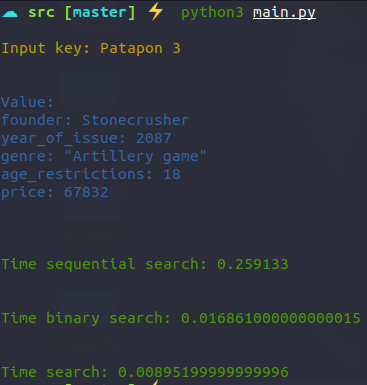
\includegraphics[width=0.6\textwidth]{res1.png}
		\caption{Последний ключ}
		\label{ref:time1}}
\end{figure}

На рис. \ref{ref:time2} произведено аналогичное сравнение, только в качестве искомого ключа
взят несуществующий. Аналогично поиск полным перебором
затрачивает больше всего времени по вышеописанной причине.

\begin{figure}[ht!]
	\centering{
		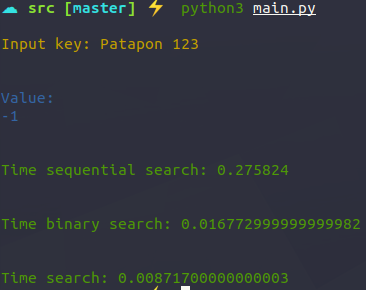
\includegraphics[width=0.6\textwidth]{res2.png}
		\caption{Несуществующий ключ}
		\label{ref:time2}}
\end{figure}

Однако не всегда поиск полным перебором дает худший результат.
На рис. \ref{ref:time3} представлен результат поиска первого значения.
Выигрыш алгоритма поиска полным перебором обосновывается тем, что он тратит
лишь одно сравнение для того, чтобы найти первый ключ, в том время, когда
бинарный поиск затрачивает гораздо больше сравнений.
Частичный анализ работает чуть медленнее, так как ему нужно
произвести дополнительное сравнение первых букв.

\begin{figure}[ht!]
	\centering{
		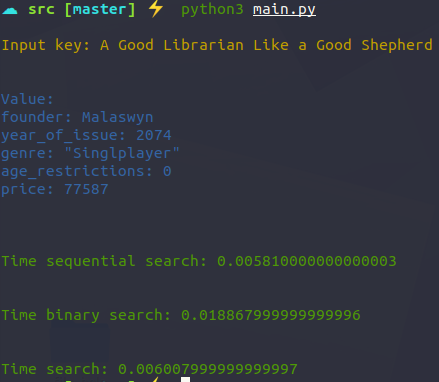
\includegraphics[width=0.6\textwidth]{res3.png}
		\caption{Первый ключ}
		\label{ref:time3}}
\end{figure}

На рис. \ref{ref:time4} представлен результат поиска произвольного ключа.
Алгоритм полного перебора работает медленнее всех.

\begin{figure}[ht!]
	\centering{
		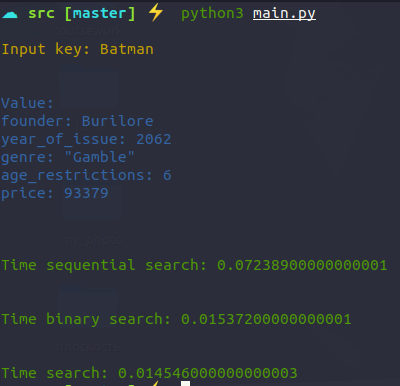
\includegraphics[width=0.6\textwidth]{res4.png}
		\caption{Произвольный ключ}
		\label{ref:time4}}
\end{figure}

\section{Вывод}

В данном разделе было произведено сравнение трех алгоритмов.
По результатам исследования было доказано, что алгоритм полного перебора
в основном работает медленнее всех, за исключением, когда ключ лежит достаточно
близко к началу.
